
\subsubsection{5.1 RQ1: Paradigm Significantly Modulates Spurious Encoding on Waterbirds}

One-way ANOVA across four paradigms $\times$ five seeds: \textbf{F = 35.99, p = 2.42 $\times 10^{-7}$}. The paradigm effect is conclusively significant.

\textbf{Table 1: Spurious/Task Probe Accuracy Ratio per Paradigm --- Waterbirds (5 seeds)}

\begin{table}[htbp]
\centering
\resizebox{\columnwidth}{!}{%
\begin{tabular}{lll}
\toprule
Paradigm & Mean Ratio & Std \\
\midrule
ERM & 1.0520 & 0.0049 \\
DINO & 1.0495 & 0.0033 \\
BarlowTwins & 1.0331 & 0.0058 \\
MoCo-v3 & 1.0273 & 0.0038 \\
\bottomrule
\end{tabular}
}
\end{table}

Individual probe accuracy estimates: ERM (spurious $\approx$ 0.931, task $\approx$ 0.884); MoCo-v3 (spurious $\approx$ 0.952, task $\approx$ 0.928); DINO (spurious $\approx$ 0.959, task $\approx$ 0.913); BarlowTwins (spurious $\approx$ 0.950, task $\approx$ 0.919).

The counterintuitive result is that MoCo-v3 --- the contrastive SSL representative --- shows the lowest spurious encoding (ratio = 1.0273), while supervised ERM shows the highest (1.0520). Augmentation-invariance theory predicts the opposite ordering.

\begin{figure}[htbp]
\centering
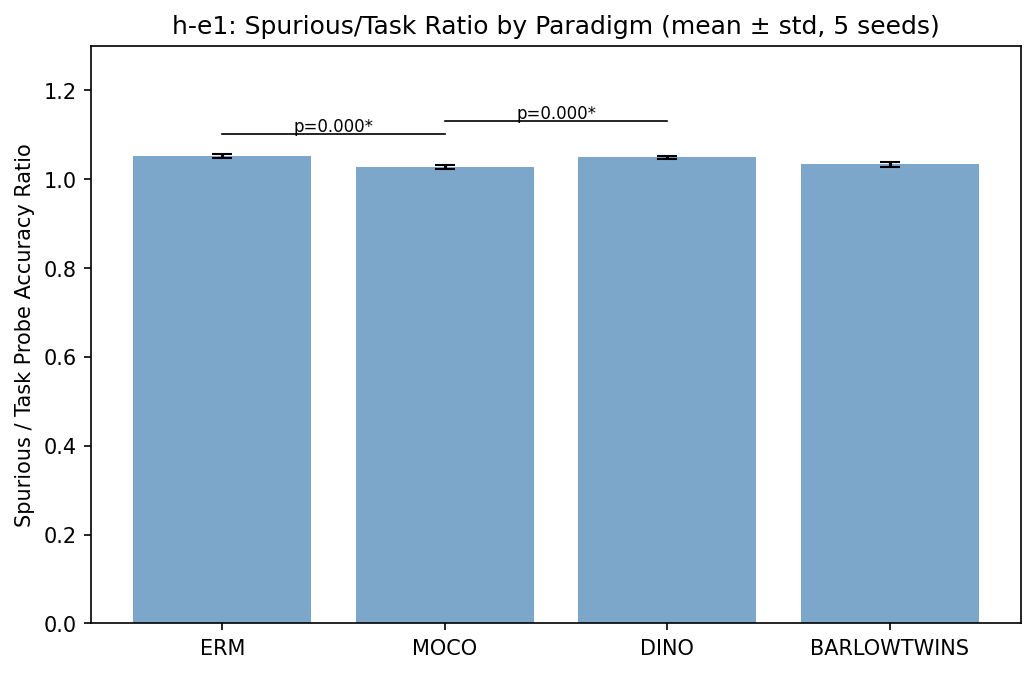
\includegraphics[width=\columnwidth]{figures/ratio_bar_waterbirds.png}
\caption{Spurious/task ratio per paradigm on Waterbirds}
\label{fig:ratio_bar_waterbirds}
\end{figure}

\textit{Figure 1: Mean spurious/task probe accuracy ratio per pretraining paradigm on Waterbirds ($\pm 1$ std, 5 seeds). Significant Bonferroni-corrected pairwise differences annotated. MoCo-v3 is lowest; ERM highest --- opposite of augmentation-invariance prediction.}

\textbf{Table 2: Pairwise Bonferroni-Corrected t-tests --- Waterbirds (n = 5 seeds per paradigm)}

\begin{table*}[htbp]
\centering
\resizebox{\dimexpr 2\columnwidth+\columnsep\relax}{!}{%
\begin{tabular}{llllll}
\toprule
Pair & t & p\_bonf & Cohen's d & Mean Diff & Gate \\
\midrule
ERM vs MoCo-v3 & 8.98 & 0.0001 & 5.68 & 0.0247 & ✅ \\
MoCo-v3 vs DINO & $-9.93$ & 0.0001 & $-6.28$ & 0.0222 & ✅ \\
ERM vs BarlowTwins & 5.60 & 0.0031 & 3.54 & 0.0188 & ✗ (diff < 0.02) \\
DINO vs BarlowTwins & 5.52 & 0.0034 & 3.49 & 0.0164 & ✗ (diff < 0.02) \\
ERM vs DINO & 0.94 & 1.000 & 0.60 & 0.0025 & ✗ \\
MoCo-v3 vs BarlowTwins & $-1.89$ & 0.572 & $-1.20$ & 0.0058 & ✗ \\
\bottomrule
\end{tabular}
}
\end{table*}

\textit{Gate criterion: p\_bonf < 0.05 AND mean\_diff $\geq$ 0.02. Cohen's d uses pooled standard deviation.}

Two pairs satisfy the full gate criterion: ERM vs MoCo-v3 (d = 5.68) and MoCo-v3 vs DINO (d = $-6.28)$. Both effect sizes are exceptional by any conventional threshold.

\textbf{ERM $\approx$ DINO:} d = 0.60, p\_bonf = 1.0. ERM and DINO are statistically indistinguishable despite their different pretraining objectives. This pattern is consistent with DINO's momentum teacher generating class-correlated soft-targets that replicate the label-correlation pressure of supervised ERM. However, alternative explanations --- such as DINO's augmentation scheme incidentally reducing variance of non-spurious features --- are not ruled out by this experiment alone.

\begin{figure}[htbp]
\centering
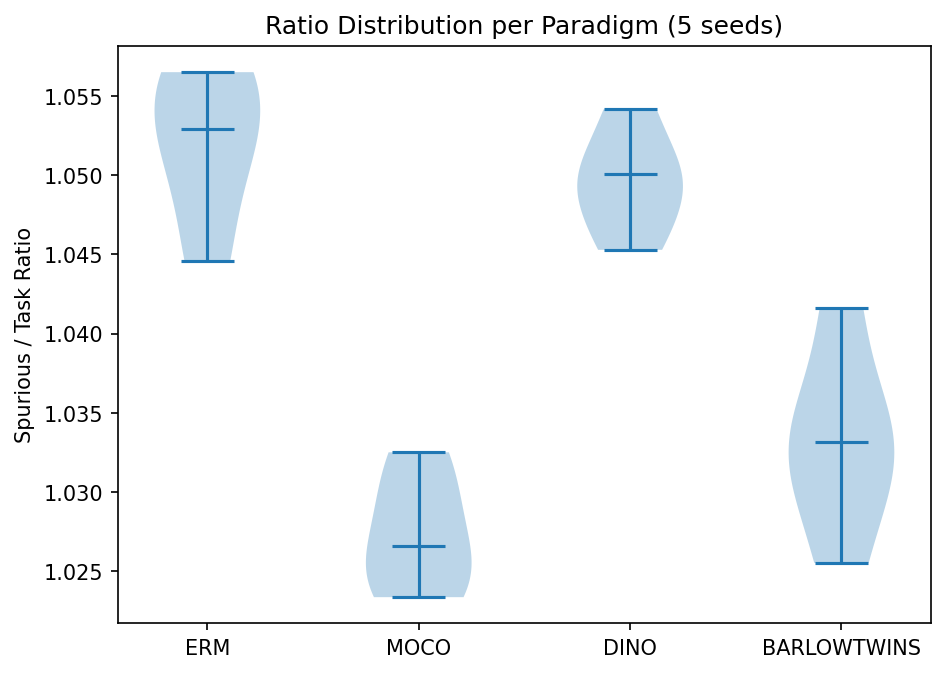
\includegraphics[width=\columnwidth]{figures/ratio_violin_waterbirds.png}
\caption{Violin plot of ratio distributions per paradigm}
\label{fig:ratio_violin_waterbirds}
\end{figure}

\textit{Figure 2: Violin distributions of spurious/task ratios across 5 seeds per paradigm (Waterbirds). MoCo-v3 is clearly separated from ERM and DINO (d = 5.68 and 6.28 respectively).}

\begin{figure}[htbp]
\centering
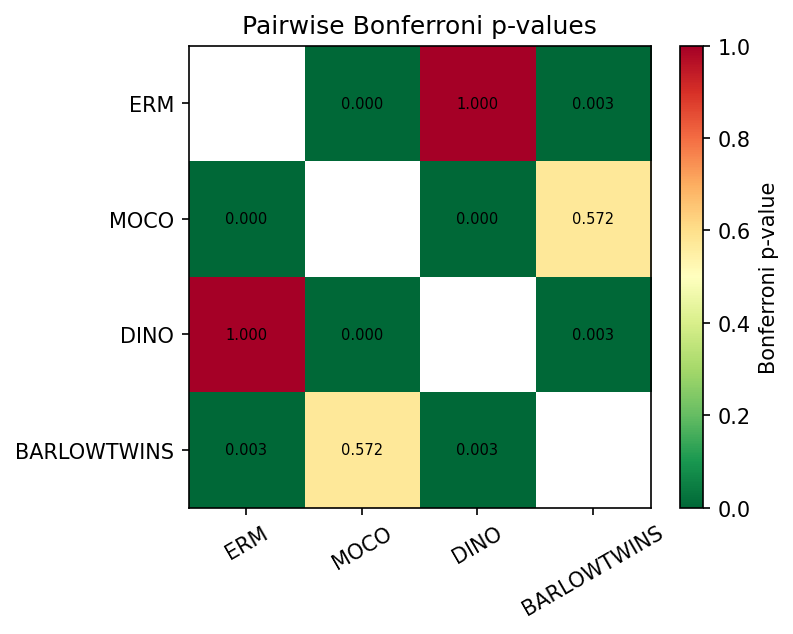
\includegraphics[width=\columnwidth]{figures/pvalue_matrix.png}
\caption{P-value matrix}
\label{fig:pvalue_matrix}
\end{figure}

\textit{Figure 3: $4\times 4$ Bonferroni-corrected p-value matrix for all pairwise paradigm comparisons on Waterbirds. Two pairs achieve p\_bonf = 0.0001: ERM vs MoCo-v3 and MoCo-v3 vs DINO.}

\begin{figure}[htbp]
\centering
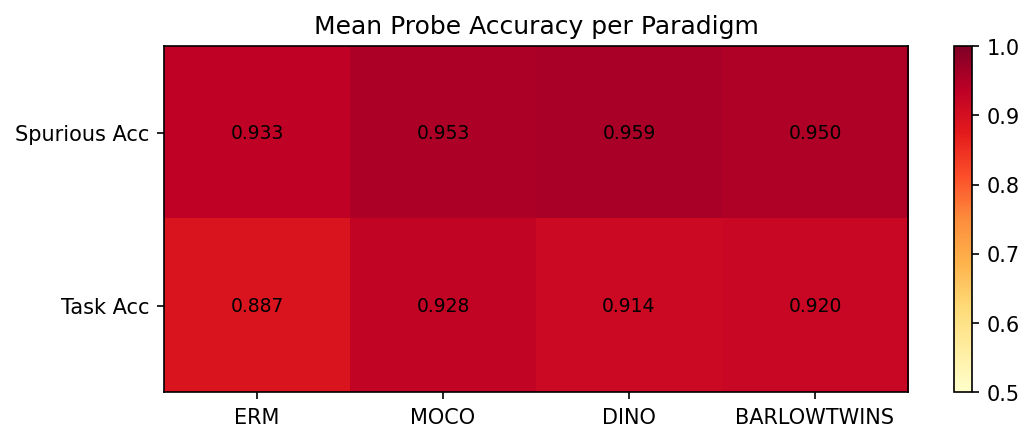
\includegraphics[width=\columnwidth]{figures/acc_heatmap.png}
\caption{Accuracy heatmap}
\label{fig:acc_heatmap}
\end{figure}

\textit{Figure 4: Heatmap of spurious and task probe accuracies (mean across seeds) per paradigm on Waterbirds. Both accuracy types differ across paradigms; ERM has the largest absolute spurious/task gap.}

\subsubsection{5.2 RQ2: Dataset-Dependent Paradigm Ranking}

\textbf{Table 3: CelebA Spurious/Task Ratios (5 seeds)}

\begin{table}[htbp]
\centering
\resizebox{\columnwidth}{!}{%
\begin{tabular}{lll}
\toprule
Paradigm & Mean Ratio & Std \\
\midrule
MoCo-v3 & 1.1976 & 0.011 \\
BarlowTwins & 1.1888 & 0.023 \\
ERM & 1.1786 & 0.010 \\
DINO & 1.1618 & 0.011 \\
\bottomrule
\end{tabular}
}
\end{table}

ANOVA on CelebA: \textbf{F = 5.51, p = 0.009}. One pairwise comparison passes the full gate criterion: MoCo-v3 vs DINO (p\_bonf = 0.005, d = 3.28, diff = 0.0359). No other pairwise comparisons pass (ERM vs MoCo-v3: p\_bonf = 0.120, d = 1.83; ERM vs DINO: p\_bonf = 0.199, d = 1.63).

CelebA ratios are uniformly higher than Waterbirds by approximately 0.14 on average. The paradigm ranking shifts substantially: MoCo-v3, which shows the lowest spurious encoding on Waterbirds (1.027), shows the highest on CelebA (1.198). DINO shifts from matching ERM on Waterbirds to the lowest ratio on CelebA.

\textbf{ERM vs MoCo-v3 on CelebA:} No significant difference. A separate directional test (h-d1) on a subset of CelebA (720 balanced samples) yields ERM mean = 1.067 $\pm$ 0.028, MoCo-v3 mean = 1.068 $\pm$ 0.013, t = 0.108, p\_two\_sided = 0.917, d = 0.068. Under either the Bonferroni-corrected pairwise test from h-e2 (p\_bonf = 0.120) or the separate directional test (p = 0.917), the ERM vs MoCo-v3 difference is not significant on CelebA. The large Waterbirds effect (d = 5.68) does not generalize to CelebA for this pair.

\begin{figure}[htbp]
\centering
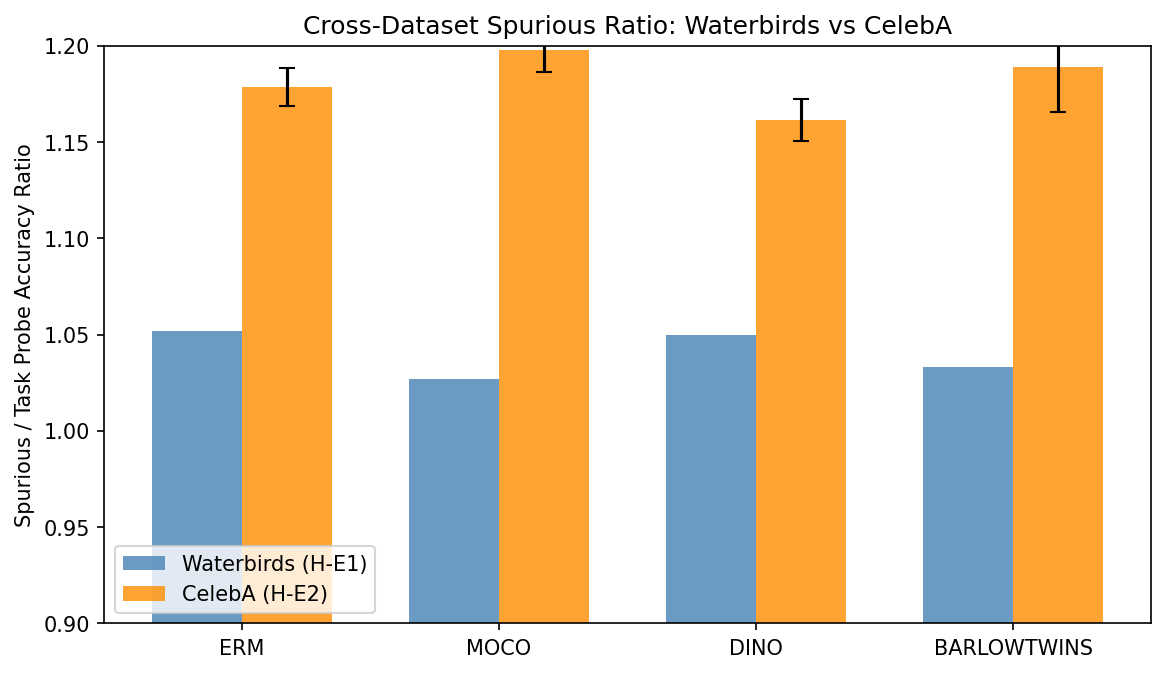
\includegraphics[width=\columnwidth]{figures/cross_dataset_bar.png}
\caption{Cross-dataset comparison}
\label{fig:cross_dataset_bar}
\end{figure}

\textit{Figure 5: Cross-dataset comparison of spurious/task ratios on Waterbirds and CelebA. The paradigm ranking reverses across datasets: MoCo-v3 is lowest on Waterbirds but highest on CelebA, while DINO matches ERM on Waterbirds but is lowest on CelebA.}

\begin{figure}[htbp]
\centering
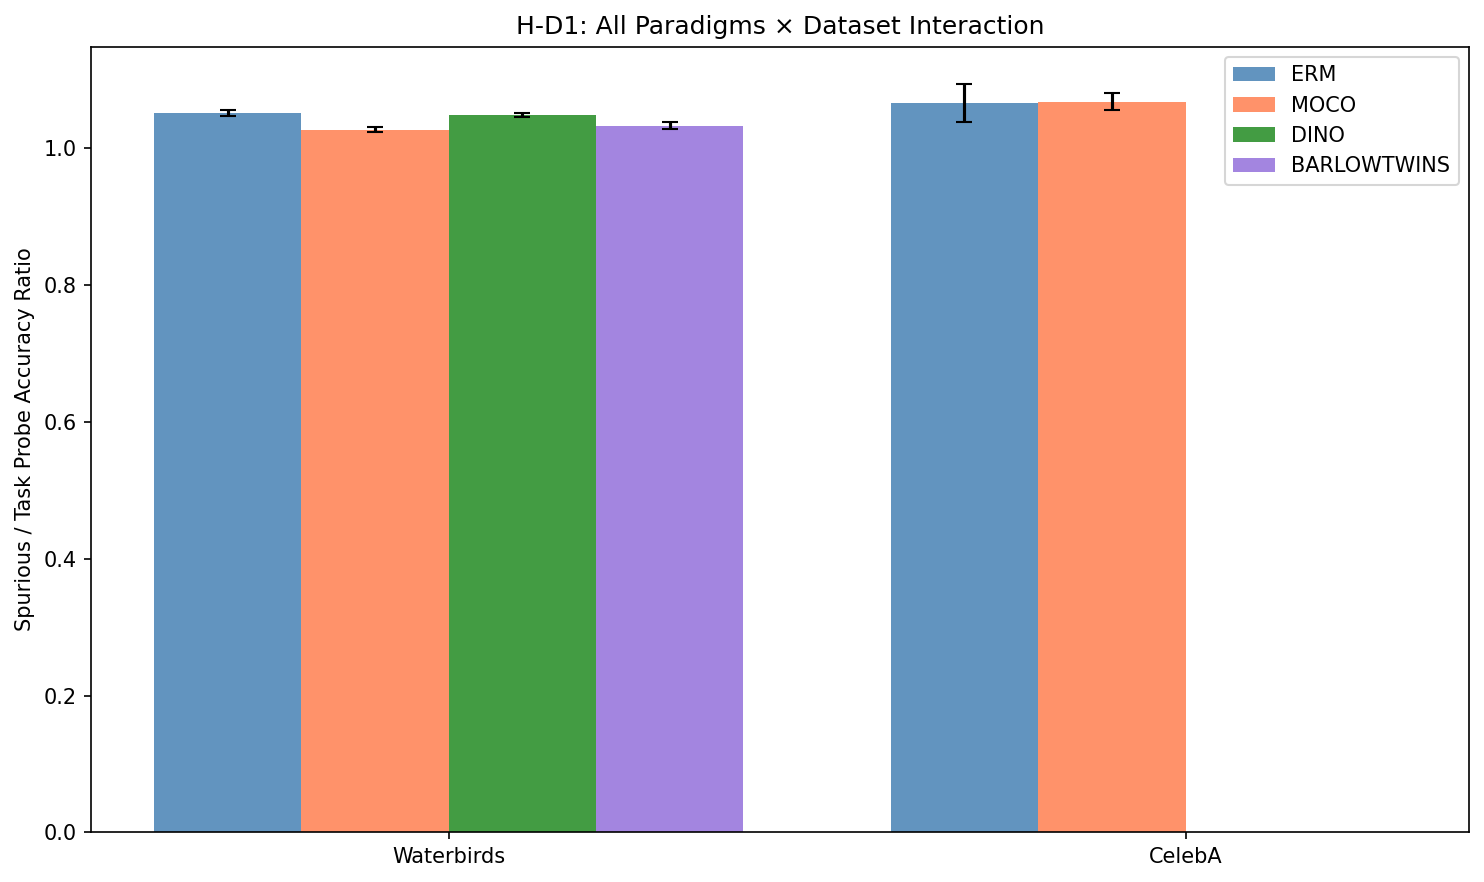
\includegraphics[width=\columnwidth]{figures/interaction_plot.png}
\caption{Interaction plot}
\label{fig:interaction_plot}
\end{figure}

\textit{Figure 6: Interaction plot for all four paradigms $\times$ two datasets. Crossing lines confirm that no paradigm consistently encodes the least spurious features across spurious attribute types.}

The ranking reversal implies that the type of spurious attribute interacts with the pretraining objective. Coarse texture spurious attributes (Waterbirds background) and demographic spurious attributes (CelebA gender) produce qualitatively different paradigm rankings. A single-dataset design would not detect this interaction.

\subsubsection{5.3 RQ3: Background-Replacement Augmentation as Functional Causal Lever}

\textbf{Mechanism verification:} pixel\_diff = 0.9656 between the background region of NoBackground and Original views (threshold = 0.05; $19\times$ margin). The background replacement is active and unambiguous.

\textbf{Full ratio statistics (5 seeds per condition, 50-epoch training):}

\begin{table}[htbp]
\centering
\resizebox{\columnwidth}{!}{%
\begin{tabular}{lll}
\toprule
Condition & Mean Ratio & Std \\
\midrule
SimCLR-Original & 1.4726 & 0.0112 \\
SimCLR-NoBackground & 1.1320 & 0.0098 \\
\bottomrule
\end{tabular}
}
\end{table}

Ratio reduction: 0.3406 (23.1\% relative reduction). Paired t-test across five seeds: t = 46.66, p = 1.26 $\times 10^{-6}$, Cohen's d = 32.4.

The spurious probe accuracy falls from approximately 0.884 (original) to approximately 0.727 (no-background), while task probe accuracy increases slightly from approximately 0.601 to approximately 0.642. The ratio reduction reflects both suppression of spurious encoding and modest improvement in task encoding.

This result confirms that explicitly removing the spurious attribute from training views causes a large reduction in spurious feature encoding in the learned representation. The absolute ratio values (1.47 and 1.13) are higher than those for the ImageNet-pretrained paradigms (1.03--1.05) because these models are trained only on Waterbirds (4,795 images) rather than on ImageNet-1k.

\textbf{Note on comparability:} SimCLR-Original and SimCLR-NoBackground are both trained from scratch on Waterbirds, not on ImageNet. Their absolute ratio values are therefore not directly comparable to the ImageNet-pretrained paradigms in Tables 1 and 3, which measure encoding in representations learned at much larger scale. The ablation comparison is valid within the from-scratch Waterbirds training setting.

